\begin{figure*}[t]
\TopFloatBoxes
\begin{floatrow}
\floatbox[\nocapbeside]{table}[0.27\textwidth]  %\FBwidth
{
\caption{\textbf{Fully and semi-supervised classification.} Legend: *Fully supervised method. $\star$Our experiments with authors' code. $\dagger$Multi-fold evaluation.}%training where average over training folds is reported (others use the full training set).
\label{t:iid_imgclus_semisup}
}
{
\scriptsize
\begin{tabular}{lc}
\toprule
& STL10 \\
\midrule
Dosovitskiy 2015~\cite{dosovitskiy2015discriminative}$\dagger$ & 74.2 \\
SWWAE 2015~\cite{zhao2015stacked}$\dagger$ & 74.3 \\
Dundar 2015~\cite{dundar2015convolutional}& 74.1 \\
Cutout* 2017~\cite{devries2017improved}& 87.3 \\
Oyallon* 2017~\cite{oyallon2017scaling}$\dagger$ & 76.0 \\
Oyallon* 2017~\cite{oyallon2017scaling}& 87.6 \\
DeepCluster 2018~\cite{caron2018deep} & 73.4$\star$ \cmt{428} \\
ADC 2018~\cite{haeusser2018associative} & 56.7$\star$ \\
DeepINFOMAX 2018~\cite{hjelm2018learning} & 77.0 \\
\methodnameshort plus finetune$\dagger$ & \textbf{79.2} \\
\methodnameshort plus finetune & \textbf{88.8} \cmt{650, 698} \\
\bottomrule
\end{tabular}}
%
\floatbox[\nocapbeside]{figure}[0.68\textwidth]  %\FBwidth
{
\caption{\textbf{Semi-supervised overclustering.} Training with \methodnameshort loss to overcluster ($k>k_{gt}$) and using labels for evaluation mapping only. Performance is robust even with 90\%-75\% of labels discarded (left and center). STL10-$r$ denotes networks with output $k=\lceil1.4r \rceil$. Overall accuracy improves with the number of output clusters $k$ (right). For further details see supplementary material. }\label{f:imgclus_variation}
}
{
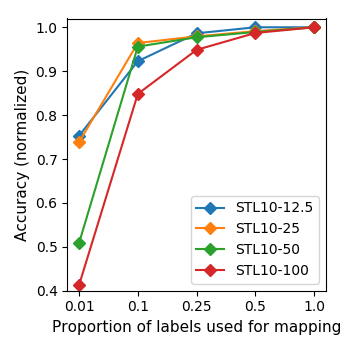
\includegraphics[width=0.215\textwidth,trim=0 0 0 1em, clip]{experiments2_files/render_vary_num_labels_stl.png}~~~%
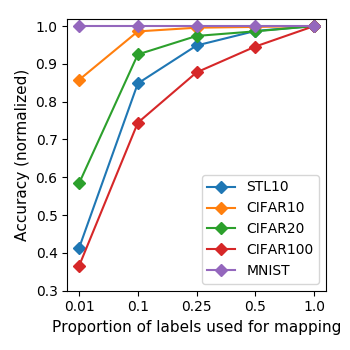
\includegraphics[width=0.215\textwidth,trim=0 0 0 1em, clip]{experiments2_files/render_vary_num_labels_all.png}~~~%
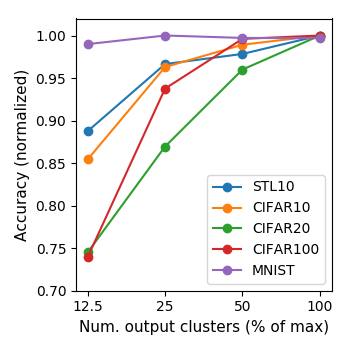
\includegraphics[width=0.215\textwidth,trim=0 0 0 1em, clip]{experiments2_files/render_vary_num_clusters.png}
}
\end{floatrow}
\end{figure*}
